\documentclass[english,11pt]{article}
\usepackage[T1]{fontenc}
\usepackage[latin9]{inputenc}
\usepackage{amsmath}
\usepackage{amsthm, amsfonts}
\usepackage{fullpage}
\usepackage[margin=1in]{geometry}
\usepackage{amssymb}
\usepackage{graphicx}
\usepackage{subcaption}
\usepackage{braket}
\usepackage{enumitem}
\usepackage{thmtools,thm-restate}
\usepackage{xcolor}
\usepackage{tikz}
\usetikzlibrary{quantikz}
\usepackage[bookmarks=false]{hyperref}
\definecolor{darkgreen}{rgb}{0,0.5,0}
\hypersetup{linktocpage=true,colorlinks=true,citecolor=red,linkcolor=darkgreen}

\usepackage[ruled,vlined,linesnumbered]{algorithm2e}

\newtheorem{theorem}{Theorem}[section]
\newtheorem{claim}[theorem]{Claim}
\newtheorem{proposition}[theorem]{Proposition}
\newtheorem{lemma}[theorem]{Lemma}
\newtheorem{corollary}[theorem]{Corollary}
\newtheorem{conjecture}[theorem]{Conjecture}
\newtheorem{remark}[theorem]{Remark}
\newtheorem{definition}[theorem]{Definition}
\makeatletter

\newcommand{\expref}[2]{{\texorpdfstring{\hyperref[#2]{#1~\ref{#2}}}{#1~\ref{#2}}}} 
\newcommand{\secref}[1]{\expref{Section}{#1}}
\newcommand{\thmref}[1]{\expref{Theorem}{#1}}
\newcommand{\clmref}[1]{\expref{Claim}{#1}}
\newcommand{\tref}[1]{\expref{Theorem}{#1}}
\newcommand{\appref}[1]{\expref{Appendix}{#1}}
\newcommand{\lref}[1]{\expref{Lemma}{#1}}
\newcommand{\corref}[1]{\expref{Corollary}{#1}}
\newcommand{\conjref}[1]{\expref{Conjecture}{#1}}
\newcommand{\pref}[1]{\expref{Proposition}{#1}}
\newcommand{\figref}[1]{\expref{Figure}{#1}}

\captionsetup[subfigure]{subrefformat=simple,labelformat=simple,listformat=subsimple}
\renewcommand\thesubfigure{(\alph{subfigure})}


%%%%%%%%%%%%%%%%%%%%%%%%%%%%%% Textclass specific LaTeX commands.
\theoremstyle{plain}
\newtheorem{thm}{\protect\theoremname}
\theoremstyle{plain}
\newtheorem{lem}[thm]{\protect\lemmaname}
\theoremstyle{remark}
\newtheorem{rem}[thm]{\protect\remarkname}

%%%%%%%%%%%%%%%%%%%%%%%%%%%%%% User specified LaTeX commands.
\usepackage{algorithmic}

\makeatother
\renewcommand{\deg}{\mathrm{deg}}
\renewcommand{\inf}{\mathrm{Inf}}
\newcommand{\Inf}{\mathrm{Inf}}
\newcommand{\maxinf}{\mathrm{MaxInf}}
\newcommand{\bs}{\mathrm{bs}}
\newcommand{\D}{\mathrm{D}}
\newcommand{\poly}{\mathrm{poly}}
\newcommand{\ui}{{\boldsymbol{i}}}
\newcommand{\eps}{\epsilon}
\usepackage{babel}
\providecommand{\lemmaname}{Lemma}
\providecommand{\remarkname}{Remark}
\providecommand{\theoremname}{Theorem}
\usepackage{color}
\newcommand{\ba}{{{a}}}
\newcommand{\R}{{\mathbb R}}
\newcommand{\N}{\mathbb{N}}
\newcommand{\C}{\mathbb{C}}
\newcommand{\pmone}{\{\pm 1\}}
\newcommand{\cbnorm}[1]{\|#1\|_{\mathrm{cb}}}
\newcommand{\Mnote}[1]{{\color{orange} {\bf Makrand: } #1}}
\newcommand{\Rnote}[1]{{\color{blue} {\bf RdW: } #1}}
\newcommand{\Nnote}[1]{{\color{red} {\bf Nikhil: } #1}}
\newcommand{\hl}[1]{\textcolor{blue}{#1}}
\newcommand{\E}{\mathbb{E}}
\newcommand{\Ef}{\E f}
\newcommand{\BZ}{\mathbf{0}}
\newcommand{\I}{\mathbb{I}}
\newcommand{\Diag}{\mathrm{Diag}}
\newcommand{\beq}{\begin{equation}}
\newcommand{\eeq}{\end{equation}}
\newcommand{\hT}{\widehat{T}}
\newcommand{\Var}{\mathrm{Var}}
\newcommand{\CP}{\mathcal{P}}
\newcommand{\NC}{\mathcal{NC}}
\newcommand{\bi}{{\boldsymbol{i}}}
\newcommand{\bj}{{\boldsymbol{j}}}
\newcommand{\comment}[1]{{}}
\newcommand{\BU}{\boldsymbol{U}}
\newcommand{\U}{\boldsymbol{U}}
\newcommand{\BA}{\mathbf{A}}
\newcommand{\BM}{\mathbf{M}}
\newcommand{\x}{\boldsymbol{x}}

\newcommand{\CA}{\mathcal A}
\newcommand{\bone}{\boldsymbol{1}}
\newcommand{\bzero}{\boldsymbol{0}}
%\newcommand{\C}{\mathbb C}
\newcommand{\tr}{\mathrm{tr}}
\newcommand{\BR}{\R}
\newcommand{\BN}{\N}
\newcommand{\CB}{\mathcal{B}}
\newcommand{\sM}{\mathsf{M}}
\newcommand{\sA}{\mathsf{A}}
\newcommand{\ind}{\mathbf{1}}
\newcommand{\op}{\mathrm{op}}
\newcommand{\BE}{\E}
\newcommand{\fhat}{\widehat{f}}
\newcommand{\del}{\partial}
\newcommand{\fix}{\mathsf{fix}}
\newcommand{\free}{\mathsf{free}}
\newcommand{\cb}{\mathrm{cb}}
\newcommand{\hf}{\widehat{f}}
\newcommand{\bb}{\boldsymbol{b}}
\renewcommand{\phi}{\varphi}
\date{} 

\begin{document}

\title{Influence in Completely Bounded Block-multilinear Forms and Classical Simulation of Quantum Algorithms}
\author{ Nikhil Bansal\thanks{\texttt{bansaln@umich.edu}. Supported in part by the NWO VICI grant 639.023.812.}\\ \small University of Michigan \and
 Makrand Sinha\thanks{\texttt{makrand@berkeley.edu}. Supported by a Simons-Berkeley postdoctoral fellowship.}\\ \small Simons Institute and UC Berkeley \and 
 Ronald de Wolf\thanks{\texttt{rdewolf@cwi.nl}. Partially supported by the Dutch Research Council (NWO/OCW), as part of the Quantum Software Consortium programme (project number 024.003.037), and through QuantERA ERA-NET Cofund project QuantAlgo (680-91-034).}\\ \small{QuSoft, CWI and U.\ of Amsterdam}
}

\maketitle
\begin{abstract}
The Aaronson-Ambainis conjecture (Theory of Computing '14) says that every low-degree bounded polynomial on the Boolean hypercube has an influential variable. This conjecture, if true, would imply that the acceptance probability of every $d$-query quantum algorithm can be well-approximated almost everywhere (i.e., on almost all inputs) by a $\poly(d)$-query classical algorithm.
We prove a special case of the conjecture: in every completely bounded  degree-$d$ block-multilinear form with constant variance, there always exists a variable with influence at least $1/\poly(d)$. In a certain sense, such polynomials characterize the acceptance probability of quantum query algorithms, as shown by Arunachalam, Bri\"et and Palazuelos (SICOMP '19). As a corollary we obtain efficient classical almost-everywhere simulation for a particular class of quantum algorithms that includes for instance $k$-fold Forrelation.
Our main technical result relies on connections to free probability theory.
\end{abstract}


\thispagestyle{empty}
\clearpage
\newpage
\setcounter{page}{1}

\allowdisplaybreaks

% !TEX root = ../arxiv.tex

Unsupervised domain adaptation (UDA) is a variant of semi-supervised learning \cite{blum1998combining}, where the available unlabelled data comes from a different distribution than the annotated dataset \cite{Ben-DavidBCP06}.
A case in point is to exploit synthetic data, where annotation is more accessible compared to the costly labelling of real-world images \cite{RichterVRK16,RosSMVL16}.
Along with some success in addressing UDA for semantic segmentation \cite{TsaiHSS0C18,VuJBCP19,0001S20,ZouYKW18}, the developed methods are growing increasingly sophisticated and often combine style transfer networks, adversarial training or network ensembles \cite{KimB20a,LiYV19,TsaiSSC19,Yang_2020_ECCV}.
This increase in model complexity impedes reproducibility, potentially slowing further progress.

In this work, we propose a UDA framework reaching state-of-the-art segmentation accuracy (measured by the Intersection-over-Union, IoU) without incurring substantial training efforts.
Toward this goal, we adopt a simple semi-supervised approach, \emph{self-training} \cite{ChenWB11,lee2013pseudo,ZouYKW18}, used in recent works only in conjunction with adversarial training or network ensembles \cite{ChoiKK19,KimB20a,Mei_2020_ECCV,Wang_2020_ECCV,0001S20,Zheng_2020_IJCV,ZhengY20}.
By contrast, we use self-training \emph{standalone}.
Compared to previous self-training methods \cite{ChenLCCCZAS20,Li_2020_ECCV,subhani2020learning,ZouYKW18,ZouYLKW19}, our approach also sidesteps the inconvenience of multiple training rounds, as they often require expert intervention between consecutive rounds.
We train our model using co-evolving pseudo labels end-to-end without such need.

\begin{figure}[t]%
    \centering
    \def\svgwidth{\linewidth}
    \input{figures/preview/bars.pdf_tex}
    \caption{\textbf{Results preview.} Unlike much recent work that combines multiple training paradigms, such as adversarial training and style transfer, our approach retains the modest single-round training complexity of self-training, yet improves the state of the art for adapting semantic segmentation by a significant margin.}
    \label{fig:preview}
\end{figure}

Our method leverages the ubiquitous \emph{data augmentation} techniques from fully supervised learning \cite{deeplabv3plus2018,ZhaoSQWJ17}: photometric jitter, flipping and multi-scale cropping.
We enforce \emph{consistency} of the semantic maps produced by the model across these image perturbations.
The following assumption formalises the key premise:

\myparagraph{Assumption 1.}
Let $f: \mathcal{I} \rightarrow \mathcal{M}$ represent a pixelwise mapping from images $\mathcal{I}$ to semantic output $\mathcal{M}$.
Denote $\rho_{\bm{\epsilon}}: \mathcal{I} \rightarrow \mathcal{I}$ a photometric image transform and, similarly, $\tau_{\bm{\epsilon}'}: \mathcal{I} \rightarrow \mathcal{I}$ a spatial similarity transformation, where $\bm{\epsilon},\bm{\epsilon}'\sim p(\cdot)$ are control variables following some pre-defined density (\eg, $p \equiv \mathcal{N}(0, 1)$).
Then, for any image $I \in \mathcal{I}$, $f$ is \emph{invariant} under $\rho_{\bm{\epsilon}}$ and \emph{equivariant} under $\tau_{\bm{\epsilon}'}$, \ie~$f(\rho_{\bm{\epsilon}}(I)) = f(I)$ and $f(\tau_{\bm{\epsilon}'}(I)) = \tau_{\bm{\epsilon}'}(f(I))$.

\smallskip
\noindent Next, we introduce a training framework using a \emph{momentum network} -- a slowly advancing copy of the original model.
The momentum network provides stable, yet recent targets for model updates, as opposed to the fixed supervision in model distillation \cite{Chen0G18,Zheng_2020_IJCV,ZhengY20}.
We also re-visit the problem of long-tail recognition in the context of generating pseudo labels for self-supervision.
In particular, we maintain an \emph{exponentially moving class prior} used to discount the confidence thresholds for those classes with few samples and increase their relative contribution to the training loss.
Our framework is simple to train, adds moderate computational overhead compared to a fully supervised setup, yet sets a new state of the art on established benchmarks (\cf \cref{fig:preview}).

%\documentclass[main]{subfiles}

\begin{document}

\section{Preliminaries}
\label{sec:preliminaries}
%\paragraph{Notation} 
\noindent
For $n \in \N$, we denote $[n] := \{1,\ldots,n\}$ and the vector with all ones as $\1_n \in \R^n$.
%\todo{Any vector $x \in \R^n$ is a column vector and its transpose is denoted by $x^T$. The entries of $x \in \R^n$ will be $x_1, \ldots, x_n$. Inequalities like $x \geq 0$ abbreviate the statement $\forall i \in [n] \, : \, x_i \geq 0$. For $i \in [n]$, we will use $e_i \in \R^n$ to denote the $i$-th standard basis vector (with a $1$ in its $i$-th entry and $0$'s anywhere else).} 
 
%\\
%\todo{When working with sets $\{S^i\}_{i=1}^N$, we denote $\displaystyle \bigtimes_{i=1}^N S^i := S^1 \times \ldots \times S^N$.} \\


\subsection{Multiplayer Games} 
A multiplayer game $G$ specifies (a) the number of players $N \in \N, N \geq 2,$ (b) a set of pure strategies $S^i = [m_i]$ for each player~$i$ where $m_i \in \N, m_i \geq 2,$ and (c) the utility payoffs for each player~$i$ given as a function $u_i: S = S^1 \times \ldots \times S^N \longrightarrow \R$. Throughout this paper, all multiplayer games considered shall have the same number of players $N$ and the same strategy sets $S^1, \ldots, S^N$. Hence, any game $G$ will be determined by its utility functions $\{u_i\}_{i \in [N]}$. The players choose their strategies simultaneously and they cannot communicate with each other. A utility function $u_i$ can be summarized by its pure strategy outcomes for player~$i$, captured as an $N$-dimensional array $\big\{ u_i(\ks) \big\}_{\ks \in S}$.

\begin{ex}
$2$-player games are better known as bimatrix games because their $2$-dimensional payoff arrays in become matrices $A,B \in \R^{m \times n}$.
\end{ex}

As usual, we allow the players to randomize over their pure strategies. Then, player~$i$'s strategy space extends to the set of probability distributions over $S^i$. We identify this set with $\Delta(S^i) := \, \Big\{ s^i = (s_k^i)_k \, \in \R^{m_i} \, \Big| \, s_k^i \geq 0 \, \, \forall k \in [m_i] \, \, \text{and} \, \sum_{k \in [m_i]} s_k^i = 1 \Big\}$ and refer to the probability distributions as mixed strategies. A tuple $\strats = (s^1, \ldots, s^N) \in \Delta(S^1) \times \ldots \times \Delta(S^N) =: \Delta(S)$ of mixed strategies is called a strategy profile in $G$\footnote{Note that in our notation, $\Delta(S)$ is not a simplex of higher dimensions itself but only the product of $N$ simplices.}. The utility payoff of player~$i$ for the strategy profile $\strats$ is defined as the player's utility payoff in expectation 
\[ u_i(\strats) := \sum_{\ks \in S} s_{k_1}^1 \cdot \ldots \cdot s_{k_N}^N \cdot u_i(\ks) \, .\]
The goal of each player is to maximize her utility.


We will abbreviate with $S^{-i}$ the set that consists of all possible pure strategy choices $\ks_{-i} = (k_1, \ldots, k_{i-1},k_{i+1}, \ldots, k_N)$ of the opponent players (resp. $\Delta(S^{-i})$ for the set of mixed strategy choices $\strats^{-i} = (s^1, \ldots, s^{i-1},s^{i+1}, \ldots, s^N)$). We will also often use $u_i(k_i,\ks_{-i})$ instead of $u_i(\ks)$ to stress how player~$i$ can only influence her own strategy when it comes to her payoff (resp. $u_i(s^i,\strats^{-i})$ instead of $u_i(\strats)$).
\begin{defn}
The best response set of player~$i$ to the opponents' strategy choices $\strats^{-i}$ is defined as $\BR_{u_i}(\strats^{-i}) :=  \argmax_{t^i \in \Delta(S^i)} \big\{ \, u_i(t^i,\strats^{-i}) \, \big\}$. 
\end{defn} 
Best response strategies capture the idea of optimal play against the other player's strategy choices. The most popular equilibrium concept in non-cooperative games is based on best responses.
\begin{defn}
A strategy profile $\strats \in \Delta(S)$ to a game $G = \{u_i\}_{i \in [N]}$ is called a \NE{} if for all player~$i \in [N]$ we have $s^i \in \BR_{u_i}(\strats^{-i})$.
\end{defn}
\noindent
By \cite{Nash48}, any multiplayer game $G$ admits at least one \NE{}.

\subsection{Positive Affine Transformations} 

The following lemma is a well-known result for $2$-player games\footnote{ See \cite[Lemma 2.1]{heyman}, \cite[Theorem 5.35]{maschler_solan_zamir_2013}, \cite[Chapter 3]{harsanyi1988general} or \cite[Proposition 3.1]{DynGT}.}:
\begin{lemma}
\label{PAT preserves lemma}
Let $(A,B)$ be a $m \times n$ bimatrix game and take arbitrary $\alpha, \beta >0$ and $c \in \R^n, d \in \R^m$. Define $A' = \alpha A + \1_m c^T$ and $B' = \beta B + d \1_n^T$.

Then the game $(A', B')$ has the same best response sets as the game $(A,B)$. Consequently, both games have the same \NE{} set.
\end{lemma}
The intuition behind this lemma is as follows:
player~$1$ wants to maximize her utility given the strategy that player~$2$ chose. A positive rescaling of $u_1$ will change the utility payoffs but will not change the sets of best response strategies. The same holds true if we add utility payoffs to $u_1$ that are only dependent on the strategy choice $s^2$ of her opponent. In the notation of bimatrix games, this intuition yields that the transformation $A \mapsto \alpha A + \1_m c^T$ does not affect the best response sets of player~$1$. The analogous result holds for player~$2$ and the transformation $B \mapsto \beta B + d \1_n^T$.

Let us generalize PATs to multiplayer games.
\begin{defn}
\label{multiplayer PAT defn}
A positive affine transformation (PAT) specifies for each player~$i$ a scaling parameter $\alpha^i \in \R, \alpha^i >0,$ and translation constants $C^i := ( c_{\ks_{-i}})_{\ks_{-i} \in S^{-i}}$ for each choice of pure strategies from the opponents. 
The PAT $H_{\textnormal{PAT}} = \big\{ \alpha^i, C^i \big\}_{i \in [N]}$ applied to an input game $G = \{u_i\}_{i \in [N]}$ returns the transformed game $H_{\textnormal{PAT}}(G) = \{u_i'\}_{i \in [N]}$ in which (only) the utility functions changed to
\begin{align}
\label{PAT transformed utilities}
\begin{aligned}
u_i' : S &\longrightarrow \R \\
\ks &\longmapsto \alpha_i \cdot u_i(\ks) + c_{\ks_{-i}}^i \, .
\end{aligned}
\end{align}
\end{defn}
We could not find multiplayer PATs defined in the literature, so we came up with the natural generalization above. As shown in Section \ref{sec:bimatrix games}, they indeed generalize the 2-player PATs from Lemma~\ref{PAT preserves lemma} to multiplayer settings. Moreover, multiplayer PATs also preserve the best response sets and \NE{} set.
\begin{lemma}
\label{multiplayer PAT preserves}
Take a PAT $H_{\textnormal{PAT}} = \big\{ \alpha^i, C^i \big\}_{i \in [N]}$ and any game $G = \{u_i\}_{i \in [N]}$. Then, the transformed game $H_{\textnormal{PAT}}(G) = \{u_i'\}_{i \in [N]}$ has the same best response sets as the input game $G$. Consequently, $H_{\textnormal{PAT}}(G)$ also has the same \NE{} set as $G$.
\end{lemma}
\begin{proof}
See \ref{sec:helpinglemmas}.
\end{proof}
PATs have found much success as a tool for simplifying an input game precisely because of this property. We want to investigate which other game transformations also preserve the best response sets or the \NE{} set. If we found more of these transformations, we could use them to, e.g., further increase the class of efficiently solvable games.

\subsection{Game Transformations}

There are various ways in which we could define the concept of a game transformation. Section~\ref{literature review} gives an overview of some definitions from the literature that are useful for different purposes. A key component of PATs are that they operate player-wise and strategy-wise, that is, they do not change the player set nor the players' strategy sets. This allows for a direct comparison of the strategic structure between a game and its PAT-transform. We argue that this is a natural desideratum for a definition of more general game transformation.

\begin{defn}
\label{def game trafo}
A game transformation $H = \{H^i\}_{i \in [N]}$ specifies for each player~$i$ a collection of functions $H^i := \Big\{ h_{\ks}^i : \R \longrightarrow \R \Big\}_{\ks \in S}$, indexed by the different pure strategy profiles $\ks$. \\
The transformation $H$ can then be applied to any $N$-player game $G = \{u_i\}_{i \in [N]}$ to construct the transformed game $H(G) = \{H^i(u_i)\}_{i \in [N]}$ where 
\begin{align}
\label{transformed pure utilities evaluation}
    H^i(u_i) : S \to \R, \quad \ks \mapsto h_{\ks}^i \big( u_i(\ks) \big) \, .
\end{align}
\end{defn}
Observe that the utility payoff of player~$i$ in the transformed game $H(G)$ from the pure strategy outcome $\ks$ is only a function of the utility payoff from \textit{that same} player in \textit{that same} pure strategy outcome of the input game~$G$.

We extend the utility functions $H^i(u_i)$ to mixed strategy profiles $\strats \in \Delta(S)$ as usual through $H^i(u_i)(\strats) := \sum_{\ks \in S} s_{k_1}^1 \cdot \ldots \cdot s_{k_N}^N \cdot h_{\ks}^i \big( u_i(\ks) \big)$. To simplify future notation, we will often use $h_{k_i,\ks_{-i}}^i$ to refer to $h_{\ks}^i$.

\begin{rem}
A multiplayer positive affine transformation $H_{\textnormal{PAT}} = \big\{ \alpha^i, C^i \big\}_{i \in [N]}$ makes a game transformation $H = \{H^i\}_{i \in [N]}$ in the above sense by setting $h_{\ks}^i : \, \, \R \to \R$, $z \mapsto \alpha^i  \cdot z + c_{\ks_{-i}}^i$.
\end{rem}
\begin{defn}
\label{defn NE preserving}
Let $H = \{H^i\}_{i \in [N]}$ be a game transformation. Then we say that $H$ universally preserves \NE{} sets if for all input games $G = \{u_i\}_{i \in [N]}$, the transformed game $H(G) = \{H^i(u_i)\}_{i \in [N]}$ has the same \NE{} set as the input game $G$.
\end{defn}

\begin{defn}
\label{defn BR preserving}
Let map $H^i$ come from a game transformation $H$. Then we say that $H^i$ universally preserves best responses if for all utility functions $u_i : S \longrightarrow \R$ and for all opponents' strategy choices $\strats^{-i} \in \Delta(S^{-i})$:
\begin{equation*}
\BR_{H^i(u_i)}(\strats^{-i}) = \argmax_{t^i \in \Delta(S^i)} \big\{ H^i(u_i)(t^i,\strats^{-i}) \big\} = \argmax_{t^i \in \Delta(S^i)} \big\{ u_i(t^i,\strats^{-i}) \big\} = \BR_{u_i}(\strats^{-i}) \, .
\end{equation*}
\end{defn}

\begin{defn}
\label{defn opponent dependence}
Let map $H^i$ come from a game transformation $H$. Then we say that $H^i$ only depends on the strategy choice of the opponents if for all pure strategy choices $\ks_{-i} \in S^{-i}$ of the opponents, we have the map identities
    \[h_{1, \ks_{-i}}^i = \ldots = h_{m_i, \ks_{-i}}^i\,: \R \to \R \, .\]
\end{defn}

\end{document}
\subsection{Proofs of \Cref{sec:ergodicity-hmc}}


% \begin{proof}
%\end{proof}

\subsubsection{Proof of \Cref{theo:irred_harris} }
\label{sec:proof-crefth-harris_0}
We first prove  \eqref{theo:irred_harris_a}.  Under the assumption that $\F$ is twice continuously
  differentiable, it follows by a straightforward induction, that for
  all $h >0$ and $q \in \rset^d$, $p \mapsto
  \Phiverletq[h][k](q,p)$, defined by  \eqref{eq:def_Phiverletq}, and $p \mapsto \gperthmc[k](q,p)$, defined by \eqref{eq:def_gperthmc}, are
  continuously differentiable and for all $(q,p) \in \rset^d \times
  \rset^d$,
\begin{equation}
  \Jac_{p,\gperthmc[T]}(q,p) =  \sum_{i=1}^{T-1}(T-i)\defEns{\nabla^2 \F \circ \Phiverletq[h][i](q,p)} \Jac_{p,\Phiverletq[h][i]}(q,p) \eqsp,
\end{equation}
where for all $q \in \rset^d$, $\Jac_{p,\gperthmc[k]}(q,p)$ ($\Jac_{p,\Phiverletq[i][h]}(q,p)$ respectively) is the Jacobian of the function $\tilde{p} \mapsto
\gperthmc[k](q,\tilde{p})$ ($\tilde{p} \mapsto
\Phiverletq[i][h](q,\tilde{p})$ respectively) at $p \in \rset^{d}$.


%  Under \Cref{assum:regOne}, $\sup_{x \in \rset^d} \normLigne{\nabla^2 \F(x)}
% \leq \constzero$ and by
% \Cref{lem:bound_first_iterate_leapfrog_a},
%  $ \sup_{(q,p) \in \rset^d \times \rset^d} \normLigne{\nabla_p \Phiverletq[h][i](q,p)} \leq (1+h \vartheta_1(h))^i$ for any $i \in \nsets$.
% Therefore for any $h >0$, $T \in \nsets$, setting $S = hT$ and using that $\tilde{h} \mapsto \vartheta_1(\tilde{h})$ is nondecreasing and greater than $1$ on $\rset_+^*$ and for any $u,s \geq 0$, $u \geq 1$, $(1+s/u)^{u-1} \leq \log(s+1) \rme^s$, we get that
Under \Cref{assum:regOne}, $\sup_{x \in \rset^d} \normLigne{\nabla^2 \F(x)}
 \leq \constzero$, therefore by \Cref{lem:inverse_1}, we have that for any $T \in \nsets$ and $h >0$,
\begin{equation}
  \label{eq:inverse_1}
 \sup_{(\q,\p) \in \rset^d \times \rset^d} \norm{\Jac_{p,\gperthmc[T]}(q,p)}
 \leq  T (\{1 + h \constzero^{1/2} \vartheta_1(h \constzero^{1/2})\}^T  -1) /h  \eqsp.
\end{equation}
%$\sup_{p \in \rset^d } \nabla_p \gperthmc[k](q,p) \leq C$.
% \begin{equation}
% \label{lem:inverse_1}
% \sup_{p \in \rset^d } \nabla_p \gperthmc[k](q,p) \leq C \eqsp.
% \end{equation}
% Then for all $q, p_1,p_2 \in \rset^d$,
% \begin{equation}
% \label{lem:inverse_1}
% \norm{\gperthmc[k](q,p_1) -\gperthmc[k](q,p_2)} \leq C \norm{p_1 - p_2} \eqsp.
% \end{equation}
For any $q \in \rset^d$, $T\in \nsets$ and $h >0$, define $\phia_{q,T,h}(p)$  for all  $p \in \rset^d$ by
\begin{equation}
  \phia_{q,T,h} (p) = p-(h/T) \gperthmc[T](q,p) \eqsp.
\end{equation}
It is a well known fact (see for example
\cite[Exercise 3.26]{duistermaat:kolk:2004}) that if
\begin{equation}
  \label{eq:inverse_1_2}
  \sup_{(q,p) \in \rset^d \times \rset^d} (h/T)\norm{ \Jac_{p,\gperthmc[T]}(q,p)} < 1 \eqsp,
\end{equation}
then for any $q \in \rset^d$, $\phia_{q,T,h}$ is a
diffeomorphism and  therefore by \eqref{eq:qk}, the same conclusion holds
for $p \mapsto \Phiverletq[h][T](q,p)$. Using \eqref{eq:inverse_1}, if $T \in \nsets$ and $h > 0$  satisfies \eqref{eq:condition-h,T-harris},
then the condition \eqref{eq:inverse_1_2} is verified and as a result \eqref{theo:irred_harris_a}.

Denoting for any $q \in \rset^d$ by $\Phiverletqi[h][T](q,\cdot) : \rset^d \to \rset$ the
continuously differentiable inverse of $p \mapsto
\Phiverletq[h][T](q,p)$ and using a change of variable with $\Phiverletqi[h][T](q,\cdot)$ in \eqref{eq:def_kernel_hmc} concludes the proof of \eqref{eq:def_kernel_hmc_false_density}.

We now show that $\Tker_{h,T}$ satisfies the condition which implies that $\Pkerhmc[h][T]$ is a \Tkernel. We first establish some estimates on the function $(q,p) \mapsto \Phiverletqi[h][T](q,p)$. By
\eqref{eq:inverse_1_2} and \eqref{eq:qk}, for any $q,p,v \in \rset^d$, there exists $\varepsilon \in \ooint{0,1}$ such that $  \normLigne{\Phiverletq[h][T](q,p)-\Phiverletq[h][T](q,v)} \geq (hT) \normLigne{\phi_{q,T,h}(p)-\phi_{q,T,h}(v)} \geq (hT) (1-\varepsilon)\norm{p-v}$ which implies that that there exists $C \geq 0$ satisfying
\begin{equation}
  \label{eq:regularity_phinverse1}
  \begin{aligned}
    \norm{\Phiverletqi[h][T](q,p)-\Phiverletqi[h][T](q,v)} &\leq (1-\varepsilon)^{-1} \norm{v-p}\eqsp, \\
    \norm{  \Phiverletqi[h][T](q,p)} &\leq C\defEns{\norm{\p} + \norm{\Phiverletq[h][T](q,0)}} \eqsp.
  \end{aligned}
\end{equation}
In addition, for $q,x,p \in \rset^d$, we have setting $\tilde{q} = \Phiverletqi[h][T](q,p)$ that
\begin{align}
  \nonumber
  \normLigne{\Phiverletqi[h][T](q,p) - \Phiverletqi[h][T](x,p)} &= \normLigne{\tilde{q} - \Phiverletqi[h][T](x, \Phiverletq[h][T](q,\tilde{q}))} \\
  \nonumber
                                                                &= \normLigne{\Phiverletqi[h][T](x, \Phiverletq[h][T](x,\tilde{q})) - \Phiverletqi[h][T](x, \Phiverletq[h][T](q,\tilde{q}))} \eqsp,
\end{align}
which implies by \eqref{eq:regularity_phinverse1} and \Cref{lem:bound_first_iterate_leapfrog_a}
that there exists $C \geq 0$ satisfying
\begin{equation}
  \label{eq:regularity_phinverse2}
  \norm{\Phiverletqi[h][T](q,p) - \Phiverletqi[h][T](x,p)} \leq C \norm{q-x} \eqsp.
\end{equation}


We now can prove that $\Tker_{h,T}$ is the continuous component of $\Pkerhmc[h][T]$. First by \eqref{eq:def_tker}, for all $\eventB \in \borelSet(\rset^d)$,
\begin{equation}
\label{eq:minoration_pseudo_density_P}
    \Tker_{h,T}(q, \eventB) \geq (2 \uppi)^{-d/2} \Leb(\eventB)
 \times \inf_{\bar{q} \in \eventB} \defEns{ \balphaacc(q,\bar{q}) \rme^{-\norm{\Phiverletqi_q(\bar{q})}^2/2}\detj_{\Phiverletqi[h][T](q,\cdot)}(\bar{q})} \eqsp,
\end{equation}
with the convention $0 \times \plusinfty = 0$ and
\begin{equation}
%  \label{eq:7}
  \balphaacc(q,\bar{q}) =  \alphaacc\defEns{(q,\Phiverletqi[h][T](q,\bar{q})),\Phiverlet[h][T](q,\Phiverletqi[h][T](q,\bar{q}))}\eqsp. 
\end{equation}
Since the function $  (q,p) \mapsto (\Phiverletq[h][T](q,p),\Phiverletqi[h][T](q,p), \detj_{\Phiverletqi[h][T](q,\cdot)}(p)) $
is continuous on $\rset^d\times \rset^d$ by \Cref{lem:bound_first_iterate_leapfrog_a}, \eqref{eq:regularity_phinverse1} and \eqref{eq:regularity_phinverse2}, and for any $q,p \in \rset^d$, $\Jac_{\Phiverletq[h][T](\q,\cdot)}(\Phiverletqi[h][T](q,p))
\Jac_{\Phiverletqi[h][t](q,\cdot)}(\p) = \operatorname{I}_n$, we get that  $\Tker_{h,T}(q,\eventB) >0$ for all $q \in \rset^d$ and all compact set $\eventB$ satisfying $\Leb(\eventB) > 0$. Therefore, using that the Lebesgue measure is regular which implies that for any $\msa \in \mcb(\rset^d)$ with $\Leb(\msa) >0$, there exists a compact set $\msb \subset\msa$, $\Leb(\msb)>0$, we can conclude that $\Pkerhmc[h][T]$ is irreducible with respect to the Lebesgue measure. In addition, we get  $\Tker_{h,T}(q,\rset^d) >0$, and therefore we obtain that $\Pkerhmc[h][T]$ is aperiodic.  Similarly we get that any compact set is $(1,\Leb)$-small.

It remains to show that for any $\eventB \in\mcb(\rset^d)$, $q \mapsto \Tker_{h,T}(q,\eventB)$ is lower semi-continuous which is a straightforward consequence of Fatou's Lemma and that for any $p \in \rset^d$, $q \mapsto (\Phiverlet[h][T](q,p), \Phiverletqi[h][T](q,p),\detj_{\Phiverletqi[h][T](q,\cdot)}(p))$ is continuous.

% We now show that all the compact sets are $(1,\Leb)$-small. Let $\eventB \subset \rset^d$ be compact.  Using
% \eqref{eq:inverse_1_2} there exists $C \geq 0$ such that for all
% $q,p,v \in \rset^d$, $ \norm{p-v} \leq C \normLigne{
%   \Phiverletq[h][T](q,p)- \Phiverletq[h][T](q,v)}$. It follows
% that for all $p \in \rset^d$, $\sup_{q \in \eventB} \normLigne{
%   \Phiverletqi[h][T](q,p)} \leq C\defEnsLigne{\norm{\p} + \sup_{q \in
%     \eventB} \normLigne{\Phiverletq[h][T](q,0)}}$. Using this upper
% bound and $\Jac_{\Phiverletq(\q,\cdot)}(\Phiverletqi_q(\p))
% \Jac_{\Phiverletqi_q}(\tilde{\p}) = \operatorname{I}_n$ in
% \eqref{eq:minoration_pseudo_density_P}, where $\operatorname{I}_n$ is
% the identity matrix, we deduce that there exists $\varepsilon >0$ such
% that for all $\eventA\in \borelSet(\rset^d)$, $\eventA \subset \eventB$,
% \begin{equation}
%   \inf_{q \in \eventB} \Pkerhmc[h][T](q, \eventA)  \geq \varepsilon \Leb(\eventA) \eqsp,
% \end{equation}
% and therefore $\eventB$ is small for $\Pkerhmc[h][T]$.
% \begin{equation}
% \norm{  \Phiverletqi_q(p_1)-  \Phiverletqi_q(p_2)} \leq C \norm{p_1-p_2} \eqsp,
% \end{equation}
% This result, \eqref{eq:def_acc_ratio}, \Cref{lem:bound_first_iterate_leapfrog} and \eqref{eq:minoration_pseudo_density_P} imply that $
% \Pkerhmc[h][T]$ is irreducible with respect to the Lebesgue measure
% and aperiodic.
% and any ball on $\rset^d$ is small.

% A straightforward adaptation of the proof of \cite[Corollary
% 2]{tierney:1994} shows that $ \Pkerhmc[h][T]$ is Harris recurrent, see \Cref{propo:harris_rec} in \Cref{sec:harr-recurr-metr}. The desired conclusion then follows from \cite[Theorem 13.0.1]{meyn:tweedie:2009}.
 % \Cref{theo:irred_harris} implies
% that for all $T \geq 0$, there exists $\hirr>0$ such that for all $h \in \ocintLigne{0,\hirr}$ and all $\q \in \rset^d$
%   \begin{equation}
% \lim_{n \to \plusinfty}    \tvnorm{\delta_\q \Pkerhmc[h][T]^n - \pi} = 0 \eqsp.
%   \end{equation}


% By \cite[Theorem 17.1.4, Theorem
% 17.1.7]{meyn:tweedie:2009}, it suffices the to prove that for all
% bounded harmonic function $\harmonic : \rset^d \to \rset$ satisfying
% \begin{equation}
%   \label{eq:def_harm}
%   \Pkerhmc[h][T]\harmonic = \harmonic \eqsp,
% \end{equation}
% %$\Pkerhmc[h][T]\harmonic = \harmonic$,
% are constant. First since $\Pkerhmc[h][T]$ is irreducible with respect
% to the Lebesgue measure and aperiodic, by \cite[Theorem
% 14.0.1]{meyn:tweedie:2009} for $\Leb$-almost all $q$ we get $\lim_{n
%   \to \plusinfty} \Pkerhmc[h][T]^n \harmonic(q) = \pi(\harmonic)$ and therefore by
% \eqref{eq:def_harm} $\harmonic(q) = \pi(\harmonic)$. Therefore we get that for all $q \in \rset^d$ by \eqref{eq:def_kernel_hmc_false_density},
% \begin{multline}
%    \Pkerhmc[h][T]^n \harmonic(q) = \pi(\harmonic)  \int_{\rset^d}  \alphaacc\defEns{(q,\tilde{p}),\Phiverlet[h][T](q,\tilde{p})} \rme^{-\norm{\tilde{p}}^2/2} \rmd \tilde{p} \\
% +   \harmonic(x) \int_{\rset^d}  \parentheseDeux{1-\alphaacc\defEns{(q,\tilde{p}),\Phiverlet[h][T](q,\tilde{p})}} \rme^{-\norm{\tilde{p}}^2/2} \rmd \tilde{p} \eqsp.
% \end{multline}
% Combining this result with \eqref{eq:def_harm}, we get for all $q \in \rset^d$
% \begin{equation}
% (\harmonic(q)-\pi(\harmonic)) \int_{\rset^d} \alphaacc\defEns{(q,\tilde{p}),\Phiverlet[h][T](q,\tilde{p})} \rme^{-\norm{\tilde{p}}^2/2} \rmd \tilde{p} = 0\eqsp.
% \end{equation}
% It follows from \Cref{lem:bound_first_iterate_leapfrog} and \eqref{eq:def_acc_ratio} that for all $q \in \rset^d$, $\harmonic(q) = \pi(\harmonic)$
% which concludes the proof.
% =======
% The proof of \ref{theo:irred_harris_b} using a change of variable with $\Phiverletqi[h][T](q,\cdot)$.

% We now show that $\Tker_{h,T}$ satisfies the condition which implies that $\Pkerhmc[h][T]$ is a \Tkernel.
% First, for all $\eventB \in \borelSet(\rset^d)$,
% \begin{equation}
% \label{eq:minoration_pseudo_density_P}
% \Tker_{h,T}(q, \eventB) \geq (2 \uppi)^{-d/2} \Leb(\eventB)
%  \times \inf_{\bar{q} \in \eventB} \defEns{\alphaacc\defEns{(q,\Phiverletqi[h][T](q,\bar{q})),\Phiverlet[h][T](q,\Phiverletqi[h][T](q,\bar{q}))} \rme^{-\norm{\Phiverletqi[h][T](q,\bar{q})}^2/2} \detj_{\Phiverletqi[h][T]}(q,\bar{q})} \eqsp,
% \end{equation}
% with the convention $0 \times \plusinfty = 0$. Since $\Phiverletqi[h][T](q,\cdot)$
% is a diffeomorphism on $\rset^d$, we get that  $
% \Tker_{h,T}(q,\eventB) >0$ for all $q \in \rset^d$ and all compact set $\eventB$ satisfying $\Leb(\eventB) > 0$. Since the Lebesgue measure is regular, this implies that $\Pkerhmc[h][T]$ is irreducible with respect to the Lebesgue measure and aperiodic.

% By Fatou's Lemma, for any $\eventB \in\mcb(\rset^d)$, $q \mapsto \Tker_{h,T}(q,\eventB)$ is lower semi-continuous.
% We now show that all the compact sets are small. Let $\eventB \subset \rset^d$ be compact.  Using
% \eqref{eq:inverse_1_2} there exists $C \geq 0$ such that for all
% $q,p,v \in \rset^d$, $ \norm{p-v} \leq C \normLigne{
%   \Phiverletq[h][T](q,p)- \Phiverletq[h][T](q,v)}$. It follows
% that for all $p \in \rset^d$, $\sup_{q \in \eventB} \normLigne{
%   \Phiverletqi[h][T](q,\p)} \leq C\defEnsLigne{\norm{\p} + \sup_{q \in
%     \eventB} \normLigne{\Phiverletq[h][T](q,0)}}$. Using this upper
% bound and $\Jac_{\Phiverletq(\q,\cdot)}(\Phiverletqi[h][T](q,\p))
% \Jac_{\Phiverletqi[h][T]}(q,\tilde{\p}) = \operatorname{I}_n$ in
% \eqref{eq:minoration_pseudo_density_P}, where $\operatorname{I}_n$ is
% the identity matrix, we deduce that there exists $\varepsilon >0$ such
% that for all $\eventA\in \borelSet(\rset^d)$, $\eventA \subset \eventB$,
% \begin{equation}
%   \inf_{q \in \eventB} \Pkerhmc[h][T](q, \eventA)  \geq \varepsilon \Leb(\eventA) \eqsp,
% \end{equation}
% and therefore $\eventB$ is small for $\Pkerhmc[h][T]$.
% >>>>>>> f8207bad5c0353bdfe37210ffc64a715e92e53ed

Finally, the last statements of \ref{theo:irred_harris_c} follows from \Cref{propo:harris_rec} in \Cref{sec:harr-recurr-metr} which implies that  $ \Pkerhmc[h][T]$ is Harris recurrent and  \cite[Theorem 13.0.1]{meyn:tweedie:2009} which implies  \eqref{eq:harris-theorem}.

\subsubsection{Proof of \Cref{theo:irred_D}}
\label{sec:proof-crefth_irred_D}
We use \Cref{coro:irred}. Indeed $\Pkerhmc[h][T]$ is
of form \eqref{eq:def_pkerb} and it is straightforward to check that it
satisfies \Cref{assumG:phi} (note that \Cref{lem:bound_first_iterate_leapfrog_a}
shows that $\Phiverlet[h][T]$ is a Lipshitz function on $\rset^{2d}$).

We now check that $\Pkerhmc[h][T]$ satisfies \Cref{assumG:irred_b}($\rassG,0,\MassG$) for all $\rassG,\MassG \in
\rset_+^*$ using \Cref{le:degree_application}.  By \eqref{eq:qk}, for all $T \in \nsets$, $h >0$, $q,p \in \rset^d$,
\begin{equation}
  \label{eq:phiverlet_gqth}
  \Phiverletq[h][T](q,p) = T
h p + g_{q,T,h}(p)
\end{equation}
where $g_{q,T,h}(p) = q - (Th^2/2) \nabla \F(q) -
h^2 \gperthmc[T](q,p)$ where $\gperthmc[T]$ is defined by \eqref{eq:def_gperthmc}. \Cref{lem:inverse_1} shows that for any $T \in \nsets$ and $h >0$, it holds that
\begin{equation}
    \label{eq:2:theo:irred_D}
\sup_{p,v,q \in  \rset^d} \frac{\norm{g_{q,T,h}(p)-g_{q,T,h}(v)}}{\norm{p - v}} \leq T h [\{1 + h \constzero^{1/2} \vartheta_1(h \constzero^{1/2} )\}^T-1] \eqsp,
\end{equation}
which implies that the condition
\Cref{le:degree_application}-\ref{propo:irred_b_item_i} is satisfied. To check that
condition  \Cref{le:degree_application}-\ref{propo:irred_b_item_ii} holds, we consider separately the two cases: $\beta <1$ and $\beta =1$.

\begin{enumerate}[label=$\bullet$, wide, labelwidth=!, labelindent=0pt]
\item Consider first the case $\beta <1$. By \Cref{assum:regOne}-\ref{assum:regOne_b},
for any $T \in \nsets$ and $h >0$, we get
\begin{equation}
\norm{\gperthmc[T](\q,\p)} \leq  T \sum_{i=1}^{T-1} \norm{\nabla \F \circ \Phiverletq[h][i](\q,\p)} \leq
\constzeroT T \sum_{i=1}^{T-1} \defEns{ 1 + \norm{\Phiverletq[h][i](\q,\p)}^{\expozero}}
 \eqsp.
\end{equation}
Hence, by \Cref{lem:bound_first_iterate_leapfrog_b}-\ref{lem:bound_first_iterate_leapfrog_1}
there exists $C \geq 0$ such that for all $R\in \rset_+^*$ and
$q,p \in \rset^d$, $\norm{q} \leq R$,
\begin{equation}
\label{eq:3:theo:irred_D}
\norm{g_{q,T,h}(p)} \leq C \defEns{1+R^{\beta} +\norm{p}^{\expozero}} \eqsp,
\end{equation}
which implies that condition \ref{propo:irred_b_item_ii} of \Cref{le:degree_application} holds for any $T \in \nsets$ and $h >0$.

\item Consider now the case $\beta =1$.  For any $T \in \nsets$, $h >0$,  $q,p \in \rset^d$ we get using \Cref{assum:regOne}-\ref{assum:regOne_a}
\begin{align}
  \norm{g_{q,T,h}(p)} &\leq \norm{q} + Th^2 \constzero  \norm{q} /2 + Th^2 \norm{\nabla U(0)} /2\\
  & \qquad \qquad +h^2 \norm{\gperthmc[T](q,p) - \gperthmc[T](q,0)} + h^2 \norm{ \gperthmc[T](q,0)} \eqsp.
\end{align}
Therefore using \Cref{lem:inverse_1}, for any $q,p \in \rset^d$, $\norm{q} \leq R$ for $R \geq 0$, for any $T \in \nsets$ and $h >0$ satisfying \eqref{eq:condition-h,T-harris}, there exists $C \geq 0$ such that
\begin{equation}
  \norm{g_{q,T,h}(p)} \leq C + h T  [ \{1+ h \constzero^{1/2} \vartheta_1(h\constzero^{1/2})\}^T-1]  \norm{p} \eqsp,
\end{equation}
showing that condition \ref{propo:irred_b_item_ii} of \Cref{le:degree_application} is satisfied.
\end{enumerate}

Therefore,  \Cref{le:degree_application} can be applied and for any $T \in \nsets$ and $h >0$ if $\beta <1$ and for any $h > 0$ and $T \in \nsets$ satisfying \eqref{eq:condition-h,T-harris} if $\beta =1$, $\Pkerhmc[h][T]$ satisfies \Cref{assumG:irred_b}($\rassG,0,\MassG$) for all $\rassG,\MassG \in
\rset_+^*$.  \Cref{coro:irred} concludes the proof of \ref{theo:irred_D_a} and \ref{theo:irred_D_b}.
The last statement then follows from   \cite[Theorem 14.0.1]{meyn:tweedie:2009}.

% Using this result and \Cref{theo:irred}, we get that for all $\rassG,\MassG  \in \rset_+^*$ there exists $\varepsilon >0$ such that
% for all $\q \in \ball{0}{\rassG}$ and $\eventA \in \borelSet(\rset^d)$,
% \begin{equation}
%   \Pkerhmc[h][T](q, \eventA) \geq \varepsilon \Leb(\eventA \cap \ball{0}{M}) \eqsp.
% \end{equation}
% \Cref{coro:irred} Combining this result and \eqref{eq:1:theo:irred_D} concludes the proof of \ref{theo:irred_D_a} and \ref{theo:irred_D_b}.

% The proof is a consequence of \Cref{lem:bound_first_iterate_leapfrog},
% \Cref{le:degree_application} and \Cref{theo:irred}.  \alain{give some
%   details}

%%% Local Variables:
%%% mode: latex
%%% TeX-master: "main"
%%% End:

\section{Open problems}
\label{sec:open}

Only a relatively small part of the protocols appearing in the quantum
cryptography literature have been analysed and proved secure within a
composable framework. To understand the security guarantees they
actually provide, and in what contexts they can be used safely, such
an analysis would however be crucial, thus representing a major task
for quantum cryptographers to be completed in the future. Here we
illustrate this task, focusing on a few areas that we consider
interesting. The first is the problem of reusing devices in device
independent cryptography (\secref{sec:open.di}). The second is
modeling quantum cryptography with non\-/asymptotic computational
assumptions (\secref{sec:open.computational}). And the third consists
in studying setup assumptions that are needed to achieve a broader
range of constructions (\secref{sec:open.other}).

\subsection{Reusing devices in device-independent cryptography}
\label{sec:open.di}


In \secref{sec:alternative.di} we modeled device\-/independent
(DI) QKD. There, the (untrusted) devices correspond to resources that
are available to the honest players. If Alice and Bob want to run
another DI-QKD protocol to generate more key once the first run is
over, they will again need all the same resources, i.e., they will
need such devices once more. Obviously, if Alice and Bob have acces to
new, fresh devices, they can run the protocol a second time with
these. However, it does not follow from that analysis that the
\emph{same} devices can be used again. In fact it has been shown by
\textcite{BCK13} that in general these devices cannot be reused a
second time: the internal memory of a device used for key (or randomness) generation may contain
information about the secret key (or random number) generated in the
first round, and the device may thus leak this information when being
reused in a second round. A secret bit may be leaked in a subtle manner.  For example, if the bit equals $0$ the device may perform the expected operations during the second round, and if the bit equals $1$ force an abort. 

Reusing devices in DI cryptography is very similar to reusing keys. In
general it cannot be done. However, in the case of keys, if one can
prove that the key is (close to) uniform and independent from the
adversary's information, then it can be recycled \--- this was covered
in \secref{sec:recycle}. The same approach could be used to recycle
devices: instead of the ideal world just consisting of a key resource,
it should as well provide access to devices that are independent of
this key as depicted in \figref{fig:open.di}.

\begin{figure}[tb]

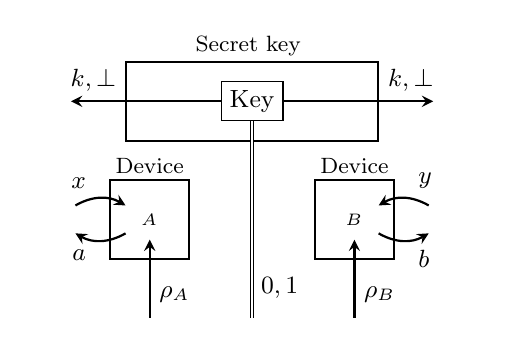
\begin{tikzpicture}[
sArrow/.style={->,>=stealth,thick},
thinResource/.style={draw,thick,minimum width=3.2cm,minimum height=1cm},
sqResource/.style={draw,thick,minimum width=1cm,minimum height=1cm},
pnode/.style={minimum width=.6cm,minimum height=.5cm}]

\small

\def\t{2.3} %1.6+.7
\def\u{.25}
\def\v{.75}
\def\w{1.3} 
\def\z{2}

\node[thinResource] (keyBox) at (0,\v) {};
\node[yshift=-1.5,above] at (keyBox.north) {\footnotesize
  Secret key $\aK$};

\node[draw] (key) at (0,\v) {Key};
\node (a1) at (-\t,\v) {};
\node (b1) at (\t,\v) {};
\node (eve) at (0,-\z) {};

\draw[sArrow] (key) to node[pos=.85,auto] {$k,\bot$} (b1.center);
\draw[sArrow] (key) to node[pos=.85,auto,swap] {$k,\bot$} (a1.center);
\draw[double] (eve.center) to node[pos=.15,auto,swap] {$0,1$} (key);


\node[pnode] (a2) at (-\t-\u,-\v) {};
\node[pnode] (b2) at (\t+\u,-\v) {};

\node[sqResource] (da) at (-\w,-\v) {$\aD_A$};
\node[yshift=-1.5,above] at (da.north) {\footnotesize
  Device};
\node[pnode] (dan) at (-\w,-\v) {};
\node[sqResource] (db) at (\w,-\v) {$\aD_B$};
\node[yshift=-1.5,above] at (db.north) {\footnotesize
  Device};
\node[pnode] (dbn) at (\w,-\v) {};

\node (eveq1) at (-\w,-\z) {};
\node (eveq2) at (\w,-\z) {};

\draw[sArrow] (eveq1.center) to node[pos=.3,auto,swap] {$\rho_A$} (dan);
\draw[sArrow] (eveq2.center) to node[pos=.3,auto,swap] {$\rho_B$} (dbn);

\draw[sArrow,bend left] (a2) to node[pos=.4,auto] {$x$} (dan);
\draw[sArrow,bend left] (dan) to node[pos=.6,auto] {$a$} (a2);
\draw[sArrow,bend right] (b2) to node[pos=.4,auto,swap] {$y$} (dbn);
\draw[sArrow,bend right] (dbn) to node[pos=.6,auto,swap] {$b$} (b2);

\end{tikzpicture}


\caption[Reusing devices]{\label{fig:open.di}An ideal world in which a
  secret key is produced by $\aK$ and new devices $\aD_A$ and $\aD_B$
  independent from $\aK$ are accessible to the players..}
\end{figure}

Unfortunately, no DI-QKD protocol has ever been shown to construct the
ideal system from \figref{fig:open.di} and it might well be impossible
to do so. But even if this is the case, it does not exclude that one
can construct an ideal system that is stronger than just the shared
secret key considered in \secref{sec:alternative.di}, e.g., one in
which the devices have some partial independence from the key or are
fully independent in certain contexts.\footnote{Context restricted
  composability is a promising research path for protocols that do not
  construct the desired ideal resource. Its investigation has been
  initiated in \textcite{JM18}, and is beyond the scope of this
  review.}

We note that weaker models such as measurement\-/device\-/independent
(MDI) QKD \--- see \secref{sec:alternative.semi} \--- do not
suffer from the same problem of device reuse as DI-QKD. The reason is
that in MDI-QKD one does not need to make any assumption about the
measurement devices at all (the adversary does the measurements for
the honest players), whereas in DI-QKD one has to assume that no
unauthorized information leaves the devices.

% This may be seen as a lack of composability: if one runs
% the protocol once in an isolated environment, the outcome remains
% secret, but if we consider a larger context where the device may be
% reused, some vital information may leak to the adversary.

% The security definitions used in device independent cryptography are
% inspired by their device dependent counterparts, e.g., the trace
% distance criterion. But unlike for the trace distance criterion, it
% has so far not been shown that these equations can be derived from a
% composable framework. In fact, it is not clear exactly what resources
% are constructed by these protocols. It is therefore an important open
% problem to develop such a framework, which enables a proper security
% analysis of device independent protocols.


\subsection{Computational security}
\label{sec:open.computational}

Computational security is a fairly unexplored area of quantum
cryptography. The main motivation for studying this is to achieve
results that are not possible with information\-/theoretic
security. For example, in \secref{sec:dqc} we mentioned a
computationally secure protocol for delegated quantum computation with
a classical client \cite{GV19}, which is believed not to be possible
with information\-/theoretic security~\cite{ACGK19}. The
computationally secure message transmission from
\secref{sec:computational} allows keys to be reused without the extra
communication required by QKD (\secref{sec:qkd}) or key recycling
(\secref{sec:recycle}) \--- and thus, without the possibility of an
adversary interrupting this communication and preventing the key from
being reused. And the work from \textcite{Unr13} discussed in
\secref{sec:mpc.ever} removes the need for a shared secret key in QKD
by using signature cards instead.

One may essentially analyze any area of cryptography with
computational security to study how assumptions needed for
information\-/theoretic security may be weakened in the computational
setting. There is however no single way to model computational
assumptions, and important open questions in the field are to identify
the (best) ways of doing this. Most frequently, one proves a
reduction, i.e., if some distinguisher can guess whether it is
interacting with the real or ideal system, then this distinguisher can
be used to solve some problem which is believed to be hard. In
\secref{sec:computational} we reviewed the finite reductions from
\textcite{BMPZ19}, in which the probability of a distinguisher $\fD$
distinguishing the real and ideal worlds is bounded by the probability
of this distinguisher being successfully used \--- as part of a new
distinguisher $\fD'$ \--- to distinguish a pseudo\-/random function
from a uniform random function; see also \textcite{Rog06} for a
discussion of reductions.

Another way to define computational security would be to define an
ideal resource that falls under the control of the adversary if she
can solve some problem believed to be hard (e.g., find a collision for
a hash function). This is essentially the ``identical-until-bad''
concept of \textcite{BR06}, but adapted to composable security instead of
game-based security. To the best of our knowledge, this paradigm remains
completely unexplored in quantum cryptography.

Other works such as \textcite{CCLVW17} bound adversaries by
circuit sizes. It is not clear how to model that in a finite,
composable framework, and is important open work.



\subsection{Other setup assumptions}
\label{sec:open.other}

When a security definition is considered ``not composable'', it often
has some (setup) assumption hard-coded in it, which is not present in
the obvious composable definition, and is therefore strictly
weaker. By modeling this assumption in a composable framework, one can
get another, equivalent composable definition. We illustrated this
in \secref{sec:alternative.memoryless} by explaining how a definition for QKD based on the accessible information, which is normally not composable, can be turned into a composable
one within a model where an adversary has no (long term) quantum
memory.

Similar techniques have been used by \textcite{Unr11} to obtain
commitments in the bounded storage model. While it follows from
\textcite{VPdR19} that coin flipping and bit commitment are impossible
in a bounded storage model without further assumptions,
\textcite{Unr11} avoids these by putting a bound on the number of
times a protocol can be run in parallel, and designing protocols that
are secure for this limited number of compositions.\footnote{This
  effectively restricts what the distinguisher/environment may do to
  distinguish the real and ideal systems, since the bound on the
  number of executions of a protocol applies to the distinguisher as
  well.} Likewise, \textcite{Pro20} has made extra setup assumptions
in the relativistic model to avoid the impossibility results of
\textcite{VPdR19}.
  
  There are numerous works where security is proved based on the assumption that adversaries are restricted. For example, adversaries cannot share entanglement in
\textcite{BCFGGOS14}, the adversaries' memory size is bounded in
\textcite{DFSS07,DFSS08}, the adversaries' memory is noisy in
\textcite{WST08,STW09,KWW12}, or adversaries can only perform local
operations on single qubits and communicate classically in
\textcite{Liu14,Liu15}. It remains open how to model these assumptions
to get composable security statements and prove in what setting such
protocols are secure. Similarly, to capture position\-/based
cryptography \textcite{Unr14} uses a model of circuits with positions in
space\-/time. Here too, it is not clear how to fit these results in a
composable framework and identify the resource that is constructed by these
protocols.


%%% Local Variables:
%%% TeX-master: "main.tex"
%%% End:









\bibliographystyle{alpha}
\bibliography{refs}
\appendix
\section{Free Probability Primer}
\label{sec:app}

There are many excellent books on free probability theory. In particular, we refer to the book \cite{NS06} for more details than the brief introduction given here.

\subsection{Preliminaries}
\label{sec:free}



\paragraph{$C^*$-algebras.} Let $\CA$ be a unital $C^*$-algebra. For our purposes, we can think of this as an algebra of bounded operators on a complex Hilbert space which is self-adjoint ($a \in \CA$
 implies $a^* \in \CA$), closed in the operator norm $\|\cdot\|$, and contains the identity ($\bone \in \CA$). A faithful trace $\phi$ on $\CA$ is a continuous linear functional $\phi: \CA \to \C$ that is  unital ($\phi(\bone)=1$), positive $\phi(aa^*) \ge 0$, and $\phi(aa^*) = 0$ iff $a=0$. 
 
 The pair $(\CA, \phi)$ where $\CA$ is a unital $C^*$-algebra and $\phi$ is a faithful trace on $\CA$ is called a $C^*$-\emph{probability space}. Elements of $\CA$ are called non-commutative random variables. An example of a $C^*$-probability space is the class $(M_n(\C), \tr_n)$, which is the class of $n \times n$ complex matrices with the normalized trace  functional defined as $\tr_n(M) = \frac{1}{n} \sum_{i=1}^n {M_{ii}}$. General $C^*$-probability spaces allow us to extend these definitions to infinite-dimensional operators, which are needed to define a non-commutative analog of independence called \emph{free independence}. Faithfulness of the trace $\phi$ then ensures that $\|a\|= \lim_{m \to \infty} \phi((aa^*)^m)^{1/2m}$ (see \cite[Proposition 3.17]{NS06}). In particular, this allows one to compute the norm $\|\cdot\|$ by using the trace method and taking higher powers of the trace functional $\phi$, as we will see below.


\paragraph{Free Independence.} Let $(\CA, \phi)$ be a $C^*$-probability space and let $\{\CA_i\}_{i=1}^n$ be unital $*$-subalgebras of  $\CA$. They are said to be \emph{free} (or \emph{freely independent}) if for all $k \in [n]$, for all indices $i_1, \ldots, i_k \in [n]$, and for all $a_1 \in \CA_{i_1}, \ldots, a_k \in \CA_{i_k}$ satisfying $\phi(a_1)=\ldots =\phi(a_k)=0$, the joint \emph{free moment},
\[ \phi(a_1 \cdots a_k) = 0\]
whenever $j_1 \neq j_2, j_2\neq j_3, \ldots, j_{k-1} \neq j_k$, that is, the free moments vanish when all the neighboring elements in the sequence $a_1, \ldots, a_k$ come from  subalgebras with distinct indices, for example, $\phi(a_1a_2a^*_1a^*_2a_3a_2)=0$.

{Non-commutative random variables $a_1, \ldots, a_n \in (\CA, \phi)$ are said to be free if the subalgebras $\{\CA_i\}_{i=1}^n$ are free, where $\CA_i$ is the unital $*$-subalgebra  generated by $a_i$ (the linear span of all monomials $a^{\eps_1}_ia^{\eps_2}_i\cdots a^{\eps_r}_i$ where $\eps_1, \ldots, \eps_r \in \{1,*\}$ and $r \in \N \cup \{0\}$). Note that the corresponding unital $C^*$-subalgebras obtained by taking the norm closure of each $\CA_i$ are also freely independent in this case (see \cite[Exercise 5.23]{NS06}).}



We remark that the set of free non-commutative random variables is an empty set if the underlying $C^*$-probability space is finite (for instance $(M_n(\C), \tr_n)$), so to find non-trivial examples one needs to work with infinite-dimensional $C^*$-probability spaces. 

\paragraph{Free Haar Unitaries and Free Groups.} Let $(\CA, \phi)$ be a $C^*$-probability space. An element $u \in \CA$ is a \emph{Haar unitary} if it is a unitary, i.e.\ $uu^*=u^*u= \bone$, and if $\phi(u^k) = 0$ for all non-zero integers $k$. A family $S = \{u_1, \ldots, u_n\} \in \CA$ in a $C^*$-probability space $(\CA, \phi)$ is called a \emph{free Haar unitary family} if each $u \in S$ is a Haar unitary and if $u_1, \ldots, u_n$ are free. For notational convenience, let us define $S^* = \{u^*_1, \ldots, u^*_n\}$ to be the set of corresponding adjoints.

One can give a very precise condition when the trace $\phi$ evaluated on a non-commutative monomial in the $u_i$'s vanishes in terms of the free group. The \emph{free group} $F_n$ with generating set $S$ is an infinite discrete group constructed as follows: a word is defined to be product of elements of $S \cup S^*$ with $\bot$ denoting the empty word that contains no symbols. A word is called reduced if it does not contain a sub-word of the form $g g^{*}$ or $g^{*} g$ for $g \in S$. Given a word that is not reduced, the process of repeatedly removing such sub-words until it becomes reduced is called reduction. The free group $F_n$ consists of all reduced words that can be built from the symbols in $S \cup S^*$ with the group operation being a product of words followed by reduction. The identity is the empty word $\bot$. 

For a $d$-tuple $\bi  = (i_1, \ldots, i_d) \in [m]^d$, let $u_{\bi}$ denote the non-commutative monomial $u_{i_1}\cdots u_{i_d}$ and write $u^*_{\bi} = (u_{\bi})^* = u^*_{i_d} \cdots u^*_{i_1}$. Let $\bi_1,\ldots, \bi_t, \bj_1, \ldots, \bj_t$ each be a $d$-tuple in $[m]^d$ and consider the degree-$2td$ non-commutative monomial $w = u^{}_{\bi_1}u^*_{\bj_1} u^{}_{\bi_2}u^*_{\bj_2}\cdots u^{}_{\bi_t}u^*_{\bj_t}$. Note that a degree-$2td$ monomial $w$ corresponds to an ordered $2td$-tuple of variables. To illustrate, if $t=1, m=3$ and $\bi_1=(1,2,3)$ and $\bj_1 = (2,2,1)$, then $w = u_{1}u_2u_3(u_2u_2u_1)^* = u_{1}u_2u_3u_1^*u^*_2u^*_2$ and corresponds to the ordered tuple $(u_1, u_2, u_3, u^*_1, u^*_2, u_2^*)$. We can also interpret $w$ as a word in the free group by applying the reduction rules. Then the next proposition follows from the definitions of free independence and Haar unitaries.

\begin{proposition} \label{prop:word}
    $\phi(w) = 1$ iff $w$ reduces to identity in the free group $F_n$, and $\phi(w) = 0$ otherwise.
\end{proposition}

 For a monomial $w$ that reduces to identity in the free group, the procedure for reducing a monomial $w$ as above first removes some adjacent pair $u_k$ (at index $i$) and $u^*_k$ (at index $j)$, then removes another adjacent pair $u_l$ and $u^*_l$ in the resulting word and so on and so forth until we reach the empty word. In particular, this reduction procedure produces a pairing of the set $[2td]$ where the index $i$ and $j$ are paired up iff the  variables at indices $i$ and $j$ in the monomial $w$ are $u_k$ and $u^*_k$ (for some $k$). Moreover, this pairing is what is called a \emph{non-crossing} pairing defined below (see \figref{fig:non-crossing}). Note that a monomial could be reduced to identity in different ways, so there could be many such non-crossing pairings for a given monomial $w$.



%\vspace{5mm}
\begin{figure}[h!]
    \centering
   \includegraphics[width=0.6\textwidth]{noncrossing.pdf}
   \caption{\footnotesize A non-crossing $*$-pairing resulting from the reduction of a word to identity in the free group}
    \label{fig:non-crossing}
\end{figure}

\paragraph{Non-crossing Pairings.}  For any even integer $n$, let $\CP_2(n)$ denote the set of all pairings of $n$, that is, the set of all partitions of $[n]$ where each block is of size two. Let $\NC_2(n) \subseteq \CP_2(n)$ denote the set of all  pairings of $[n]$ that are non-crossing,\emph{ i.e.} pairings  which do not contain blocks $\{i_1,i_3\}, \{i_2, i_4\}$ such that $i_1 < i_2 < i_3 < i_4$. 

For integers $d,m$, we divide the set $[2dm]$ into $2m$ consecutive blocks of $d$ elements each and color consecutive blocks alternatively with red and blue. Formally, for $i \in [2m]$, the elements $\{(i-1)d+1,\ldots, id\}$ are colored red if $i$ is odd and blue if $i$ is even. We define $\NC_2^*(d,m) \subseteq \NC_2(2dm)$ to be the set of those non-crossing pairings of $[2dm]$ which only pair up elements of different colors. We call any pairing in $\NC_2^*(d,m)$ a $*$-pairing.

We shall need the following combinatorial fact about the number of $*$-pairings (see \cite[Corollary 3.2]{KS05}).

\begin{lemma}\label{lem:catalan-fuss}
    For all $d, m$, the number of $*$-pairings  $|\NC_2^*(d,m)|$ equals the Fuss-Catalan number
    \[ 
    C_{d,m} = \frac{1}{m}\binom{m(d+1)}{m-1} = O\left(\frac{(d+1)^{m(d+1)}}{\left(d+\frac1m\right)^{md+1}}\right).
    \] 
\end{lemma}




\subsection{Proofs of \lref{thm:trace} and \thmref{thm:op-norm}}



\begin{proof}[Proof of \lref{thm:trace}]
    Writing $u^*_\bi = (u_\bi)^*$ for a tuple $\bi$ and using linearity of $\phi$, we have that 
    \[ 
    \phi[p(u_1, \ldots, u_t) (p(u_1, \ldots, u_t))^*] =  \sum_{|\bi|,|\bj| \le d} c_{\bi}c_{\bj} \phi(u_{\bi}u^*_{\bj}).
    \]
    From \pref{prop:word}, the term $\phi(u_{\bi}u^*_{\bj})$ is 1 iff $u_{\bi}u^*_{\bj}$ reduces to identity in the free group $F_t$ with generators $u_1, \ldots, u_t$. For the right-hand side above, this only happens when $\bi=\bj$ and thus these are the only non-zero terms. Thus, 
    \[ \phi[p(u_1, \ldots, u_t) (p(u_1, \ldots, u_t))^*] =  \sum_{|\bi| \le d} |c_{\bi}|^2. \qedhere\]
\end{proof}

Below we present the argument of Kemp and Speicher \cite{KS05}. Our exposition follows their proof closely but we adapt it to our context.
\begin{proof}[Proof of \thmref{thm:kemp-speicher}]
     We have that $\|p\| = \lim_{m \to \infty} \left(\phi((pp^*)^m)\right)^{1/(2m)}$ by the faithfulness of the trace $\phi$. Writing $u^*_\bj = (u_\bj)^*$ for a tuple $\bj$, we can compute 
    \begin{align*}
         \phi((pp^*)^m) = \sum_{\substack{|\bi_1|=\ldots=|\bi_m|=d\\|\bj_1|=\ldots=|\bj_m|=d}} c_{\bi_1}\cdots c_{\bi_m}c_{\bj_1}\cdots c_{\bj_m} \phi(u^{}_{\bi_1}u^*_{\bj_1} \cdots u^{}_{\bi_m}u^*_{\bj_m}).
    \end{align*}
    
    Since $u_1, \ldots, u_t$ are free Haar unitaries, \pref{prop:word} implies that $\phi(u^{}_{\bi_1}u^*_{\bj_1} \cdots u^{}_{\bi_m}u^*_{\bj_m})$ is 1 iff the word $u^{}_{\bi_1}u^*_{\bj_1}\cdots u^{}_{\bi_m}u^*_{\bj_m}$ reduces to identity in the free group $F_t$, and is 0 otherwise. Moreover, if the word corresponding to the index $(\bi_1,\bj_1, \ldots, \bi_m,\bj_m)$ reduces to identity, then there exists a $*$-pairing $\pi \in \NC_2^*(d,m)$ which matches only variables with the same indices. We call any such $*$-pairing $\pi$ consistent with the $2dm$-tuple $(\bi_1,\bj_1, \ldots, \bi_m,\bj_m)$ and denote this by the indicator function $\ind[\pi, \bi_1,\bj_1, \ldots, \bi_m,\bj_m]$.
    
    The above implies that we may bound 
    \[ \phi(u^{}_{\bi_1}u^*_{\bj_1} \cdots u^{}_{\bi_m}u^*_{\bj_m})  \le \sum_{\pi \in \NC^*_2(d,m)} \ind[\pi, \bi_1,\bj_1, \ldots, \bi_m,\bj_m],\]
    where the inequality occurs because there could be multiple $*$-pairings consistent with a tuple. We thus have that 
    \begin{align*}
         \phi((pp^*)^m) &\le \sum_{\substack{|\bi_1|=\ldots=|\bi_m|=d\\|\bj_1|=\ldots=|\bj_m|=d}} c_{\bi_1}\cdots c_{\bi_m}c_{\bj_1}\cdots c_{\bj_m} \sum_{\pi \in \NC^*_2(d,m)} \ind[\pi, \bi_1,\bj_1, \cdots, \bi_m,\bj_m]\\
         &= \sum_{\pi \in \NC^*_2(d,m)}  \sum_{\substack{|\bi_1|=\ldots=|\bi_m|=d\\|\bj_1|=\ldots=|\bj_m|=d}} c_{\bi_1}\cdots c_{\bi_m}c_{\bj_1}\cdots c_{\bj_m} \ind[\pi, \bi_1,\bj_1, \cdots, \bi_m,\bj_m].
    \end{align*}
    
    If a term corresponding to a fixed $*$-pairing $\pi$ is non-zero, then the list of indices $(\bi_1, \ldots, \bi_m)$ is the same as $(\bj_1, \ldots, \bj_m)$ up to the exact ordering. Let us relabel $(\bi_1, \ldots, \bi_m) = (a_1, \ldots, a_{dm})$ and $(\bj_1, \ldots, \bj_m) = (b_1, \ldots, b_{dm})$ and let $c_{a_1, \ldots, a_{dm}} = c_{\bi_1}\ldots c_{\bi_m}$ and $c_{b_1, \ldots, b_{dm}} = c_{\bj_1}\cdots c_{\bj_m}$. Since $\pi$ gives a non-crossing bijection between the two lists $(a_1, \ldots, a_{dm})$ and $(b_1,\ldots, b_{dm})$, it holds that $c_{b_1, \ldots, b_{dm}} = c_{\pi(a_1),\ldots, \pi(a_{dm})}$. Thus, the above sum is
    \begin{align*}
        \ \phi((pp^*)^m) &\le \sum_{\pi \in \NC^*_2(d,m)}  \sum_{a_1, \ldots, a_{dm}} c_{a_1, \ldots, a_{dm}} c_{\pi(a_1),\ldots, \pi(a_{dm})}\\
        \ &\le \sum_{\pi \in \NC^*_2(d,m)} \left(\sum_{a_1, \ldots, a_{dm}} |c_{a_1, \ldots, a_{dm}}|^2\right)^{1/2}
        \left(\sum_{a_1,\ldots, a_{dm}} |c_{\pi(a_1),\ldots, \pi(a_{dm})}|^2\right)^{1/2},
    \end{align*}    
     where the inequality follows from Cauchy-Schwarz. The two internal summations are exactly the same since the summation is over all $dm$ tuples of indices and $\pi$ is a bijection. Switching back to the old indexing scheme, the internal summation then equals 
     \[  \sum_{a_1, \ldots, a_{dm}} |c_{a_1, \ldots, a_{dm}}|^2 = \sum_{\substack{|\bi_1|=\ldots=|\bi_m|=d}} |c_{\bi_1}\cdots c_{\bi_m}|^2 = \left(\sum_{|\bi|=d} |c_{\bi}|^2\right)^m.\] 
    Overall, we have
     \begin{align*}   
        \  \phi((pp^*)^m) &\le |\NC^*_2(d,m)|\left(\sum_{|\bi|=d} |c_{\bi}|^2\right)^m.
    \end{align*}
    Using \lref{lem:catalan-fuss} to bound the number of $*$-pairings,
    \[ |\NC^*_2(d,m)| = C_{d,m} = \frac{1}{m}\binom{m(d+1)}{m-1} = O\left(\frac{(d+1)^{m(d+1)}}{\left(d+\frac1m\right)^{md+1}}\right).\]
    Thus, taking the $m$-th root in the limit $m \to \infty$ yields
    \[ \|p\|^2 = \lim_{m \to \infty}  \phi((pp^*)^m)^{1/m} = \frac{(d+1)^{d+1}}{d^d}\left(\sum_{|\bi|=d} |c_{\bi}|^2\right) \le e(d+1) \left(\sum_{|\bi|=d} |c_{\bi}|^2\right).\]
    This completes the proof of the theorem.
\end{proof}






\end{document}
